% $Id$

\chapter{Regression dataset}
\minitoc

This chapter will describe the steps necessary to perform a regression using PRoNTo. These are similar to the ones in the previous chapter, thus, the reader is advised to complete the tutorial in Chapter \ref{sec:Block_design_fMRI_dataset} before moving on, since the explanation of some steps will be less descriptive. The dataset used in this chapter can be found on PRoNTo's website \url{http://www.mlnl.cs.ucl.ac.uk/pronto/prtdata.html} (data set 3).


\section{GUI analysis}
As in Chapter \ref{sec:Block_design_fMRI_dataset}, the analysis of the data will start with the PRoNTo's GUI. Please create a folder in your computer to store the results and type `prt' or `pronto' on the MATLAB command window. This will open the main interface of PRoNTo (see Figure \ref{fig:mainInterface} in the previous chapter).


%----------------------------------------------------------------------

\subsection{Data \& Design}

\begin{itemize}

	\item In PRoNTo's main window, click on `Data \& Design'. Like in the previous chapter, browse the directory in which to save the PRT structure (saved as `PRT.mat');
	
	\item In the panel `Groups', click on `Add' and provide a name to the group, e.g. `Aged';

	\item Unlike the previous chapter, all the images in the dataset correspond to different subjects; therefore, click on the `Scans' tick box. This will lock the `Subjects/Scans' field, allowing you to skip to the third field;
	
	\item In the `Modalities' panel, click on `Add' and provide a name for the modality, e.g. `fMRI';
	
	\item Load all the image files available in the directory (IXIdata/aged/Guys/). You can select all the files by using the right mouse button and clicking on the option `Select All'. When all the images are selected, click on the `Done' button;
 
    \item Into the `Regression targets' field, write (or paste) the list of target values available in the `Age\_old\_Guys' file (IXIdata/aged/). The final window should look like to the Figure \ref{fig:specifyModalityReg}. Press `OK'; 

        \begin{figure}[h!]
            \begin{center}
                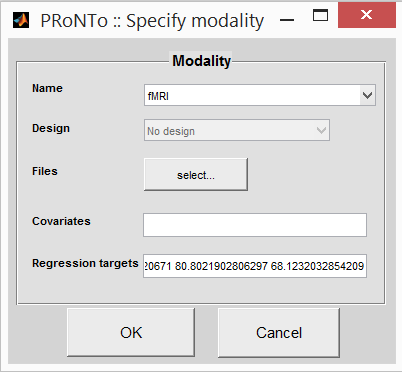
\includegraphics[scale=0.75]{images/Tutorial/regression/specifyModalityReg.png}
            \end{center}
            \caption{`Specify modality' GUI.}
            \label{fig:specifyModalityReg}
        \end{figure}

	 \item In the `Masks' field, on the bottom left of the `Data and design' window, select the `SPM\_mask\_noeyes' mask for the specified modality. The mask is available in the path where you have installed PRoNTo (PRoNTo/masks/);
    
     \item The `Data and design' window should look similar to Figure \ref{fig:dataDesignFinal}. Click on the `Save' button to create `PRT.mat' file with the structure containing the information that has been previously specified. If no errors are shown in the MATLAB command, leave the `Data and design' window by clicking `Quit'.
     
     \begin{figure}[h!]
            \begin{center}
                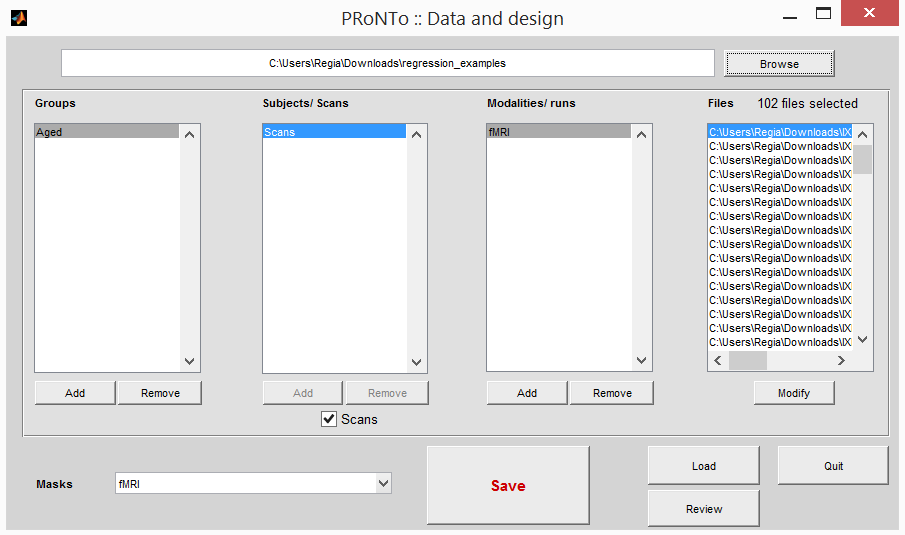
\includegraphics[scale=0.75]{images/Tutorial/regression/dataDesignFinal.png}
            \end{center}
            \caption{`Data and design' GUI final configuration.}
            \label{fig:dataDesignFinal}
        \end{figure}


\end{itemize}

%----------------------------------------------------------------

\subsection{Prepare feature set}


\begin{itemize}

	\item In PRoNTo's main window, click on `Prepare feature set' and a new window will open, `Prepare feature set' (see Figure \ref{fig:prepareFeature} in the previous chapter);   

	\item Select the `PRT.mat' file previously created in the `Data \& Design' step and another window will open, `Specify modality to include' (Figure \ref{fig:specifyModality2}). There is no need to change anything for this example. Just click on the `Done' button;
	
	\begin{figure}[h!]
            \begin{center}
                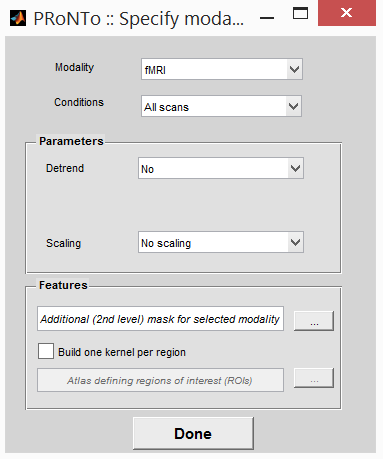
\includegraphics[scale=0.75]{images/Tutorial/regression/specifyModality2.png}
            \end{center}
            \caption{`Specify modality to include' GUI.}
            \label{fig:specifyModality2}
        \end{figure}
	
	\item In the `Prepare feature set' window, provide a name to the feature set, e.g. `Scalar\_Momentum'; and click on `Build Kernel / data matrix' to build the feature set and kernel;
	
\end{itemize}

%----------------------------------------------------------------

\subsection{Specify model}
\begin{itemize}

    \item In PRoNTo's main window, click on `Specify model' and a new window will open, `Specify model' (see Figure \ref{fig:specifyModel} in the previous chapter);

   	\item Select the `PRT.mat' file and provide a name to the model, e.g. `KRR';

    \item Select one of the `Feature Set' previously defined. In this case, there is only one: `Scalar\_Momentum';

	\item Leave the option `Use kernels' tick box as it is, i.e. `Yes';
	
	\item Select the `Regression' model type and click on the `Select subjects/scans` button. This will open a new window, `Specify subjects/scans to regress', click on the `Select all' button to use all the scans for the regression  (Figure \ref{fig:specifySubjects});
	

        \begin{figure}[h!]
            \begin{center}
                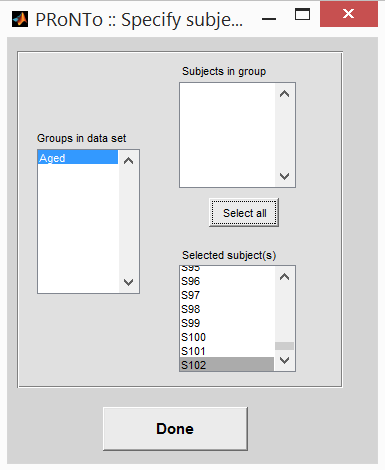
\includegraphics[scale=0.75]{images/Tutorial/regression/specifySubjects}
            \end{center}
            \caption{`Specify subjects/scans to regress' GUI.}
            \label{fig:specifySubjects}
        \end{figure}
        
     \item Select the `Kernel Ridge Regression' option, in the Machine field;
     
	 \item Leave the option `Optimize hyper-parameter' tick box unchecked and `Cross-Validation Scheme' (internal loop) as it is; 
	
	\item Select the `Leave One Subject Out' cross-validation scheme (external loop);
	
	\item In the `Data operations' box, select the `Mean centre features using training data' option. The final `Specify model' window should look similar to the Figure \ref{fig:specifyModelFinal}. Click on the `Specify and run model' button;
	     

        \begin{figure}[h!]
            \begin{center}
                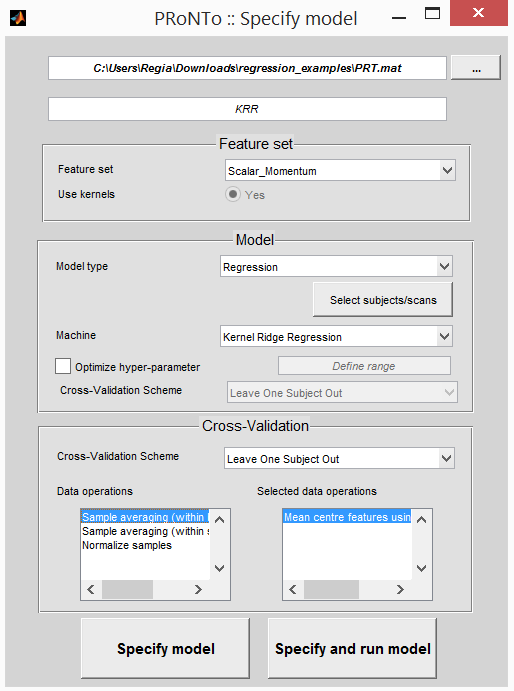
\includegraphics[scale=0.75]{images/Tutorial/regression/specifyModelFinal.png}
            \end{center}
            \caption{`Specify model' GUI final configuration.}
            \label{fig:specifyModelFinal}
        \end{figure}

    \item Repeat the process two times using the other two machines. To do this, just follow the same steps in this section, but select the other options in the `Machine' drop-down list (`Relevance Vector Regression' and `Gaussian Process Regression') and give different names to the each model.

\end{itemize}

%----------------------------------------------------------------------------

\subsection{Display results}
\label{sec:display_results_reg}
\begin{itemize}

    \item In PRoNTo's main window, click on `Display results' and select the `PRT.mat' file. This will open the main results window similar to the Figure \ref{fig:resultsReg};

        \begin{figure}[h!]
            \begin{center}
                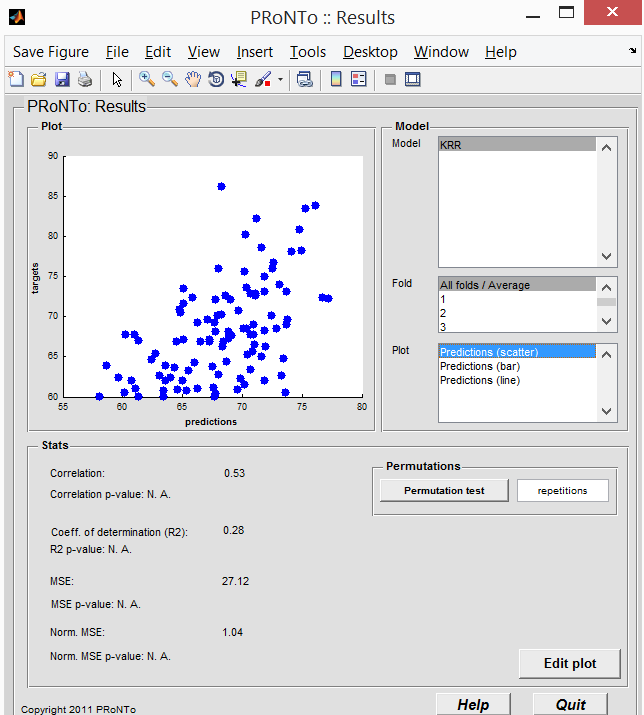
\includegraphics[scale=0.75]{images/Tutorial/regression/resultsReg.png}
            \end{center}
            \caption{`Results' GUI.}
            \label{fig:resultsReg}
        \end{figure}

    \item In the `Results' window, one can select the different regression models in the `Model' list on the upper right region. This will show the results obtained using each one of the regression models.
\end{itemize}


%=====================================================



%=====================================================

\section{Batch analysis}

In this section, the previous experiment will be repeated using the `\texttt{matlabbatch}' system. The reader is advised to complete the tutorial in Section \ref{sec:Batch_analysis_svm} before continuing, since the explanation of each step will be less descriptive.

Once again, to analyse the data, create a new directory in which to save the results of the analysis. On the main interface of PRoNTo click on the `Batch' button to open the `{\tt matlabbatch}'. Alternatively, type `prt\_batch' in the MATLAB prompt.

\subsection{Data \& Design}
\begin{itemize}

    \item Click on `Data \& Design' in the PRoNTo menu (see Figure \ref{fig:batchData} in the previous chapter);
    
    \item In the `Directory' field, select a directory where the `PRT.mat' file will be saved;
    
    \item In the `Groups' field:
 	
		\begin{itemize}
		
		\item Add one group;
		
		\item In the field `Name', provide a name without spaces for this group, e.g. `Aged';

    	\item In the field `Select by', select the `Scans' option and add a new modality. For more information on the Scans option please consult Chapter \ref{chap:DataDesign};	
        	
    	\item Provide a name for this modality, e.g. `fMRI'; select the image files available in the `aged/Guy' directory of the IXI dataset and write (or paste) the regression targets\footnote{Available in the `Age\_old\_Guys' file (IXIdata/aged/)} in the `Regression targets (per scans)' field;
    	
    	\item Leave `Covariates' field as default. The batch editor should look similar to the Figure \ref{fig:batchGroup};

        \begin{figure}[h!]
            \begin{center}
                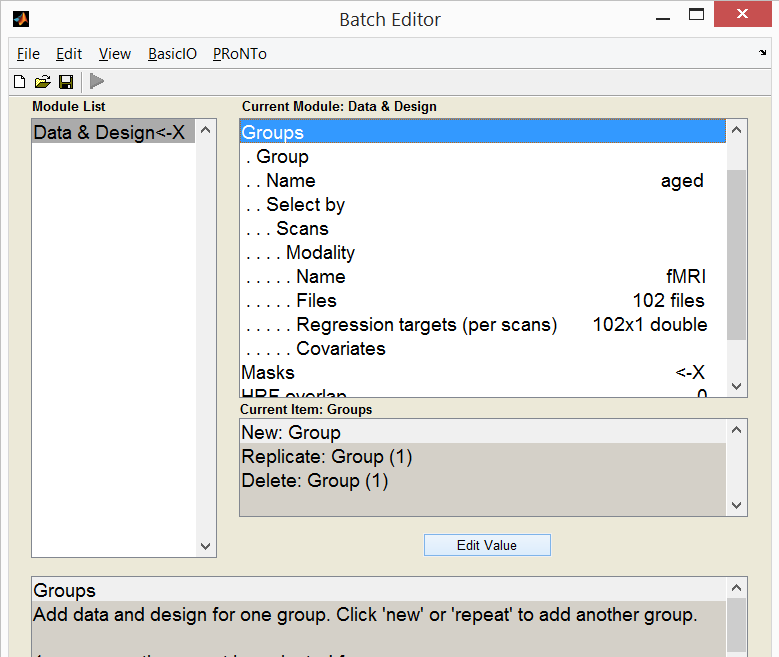
\includegraphics[scale=0.75]{images/Tutorial/regression/batchGroup.png}
            \end{center}
            \caption{Data and design module in {\tt matlabbatch}.}
            \label{fig:batchGroup}
        \end{figure}    	
    
		\item In the `Masks' field, add a new modality and provide the same modality name, `fMRI'; and select the `SPM\_mask\_noeyes' mask available in the path where you have installed PRoNTo (PRoNTo/masks/). The name of the modality here has to be exactly the same as in `Modalities', otherwise it will not work;       
        
    \item Leave the `HRF overlap' and the `HRF delay' fields as default;
	
	\item In the `Review' field, select `Yes' if you would like to review your data and design in a separate window. Otherwise, leave as it is, i.e. `No'.

\end{itemize}

\end{itemize}
%---------------------------------------------------------------

\subsection{Feature set/Kernel}

\begin{itemize}

    \item Click on the `Feature set / Kernel' option on PRoNTo's {\tt matlabbatch} menu (see Figure \ref{fig:batchFeature} in the previous chapter);
    
     \item With `Load PRT.mat' field selected, click on the `Dependency' button to associate the `PRT.mat' file created in the previous `Data \& Design' step or click on the `Select files' button to browse where `PRT.mat' file was saved;

    \item Provide a name to the `Feature/kernel' set, e.g. `Scalar\_Momentum';
    
    \item Add one modality and select the modality name with the `Dependency' button\footnote{Or type it in manually, `fMRI', but the name needs to be {\it exactly} the same as the one specified in the `Data \& Design' module.}(Data \& Design:Mod\#1 name);
	
		\begin{itemize}
	
	\item In the `Scans/Conditions' field, select `All scans' option;
	
	\item In the `Voxels to include' field, select `All voxels' option, this means we are not entering with an additional second-level mask;
	
	\item In the `Detrend' field, select the `None' option;
	
	\item In the `Scale input scans' field, select the `No scaling' option;
	
	\item Leave `Load Atlas' as default. After all these steps, the batch editor should look similar to the one in Figure \ref{fig:batchModalityReg};
	
	\begin{figure}[h!]
	\centering
		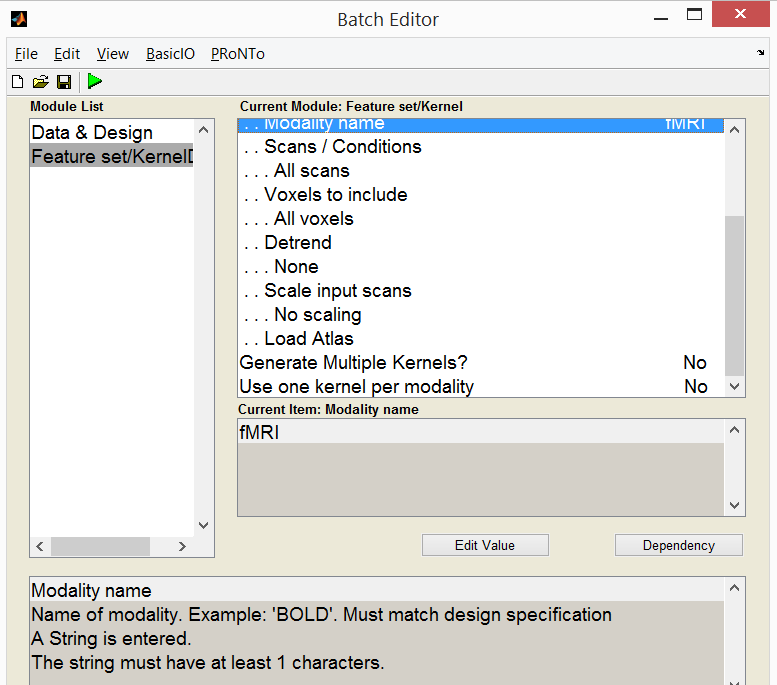
\includegraphics[scale=0.75]{images/Tutorial/regression/batchModalityReg.png}
	\caption{Feature set / Kernel module. Selected parameters in the Modality option.}
	\label{fig:batchModalityReg}
\end{figure}
	
	\end{itemize}
	   
    \item Leave the `Generate Multiple Kernels' and the `Use one kernel per modality' fields as default.
    
\end{itemize}

%----------------------------------------------------------------------

\subsection{Specify model (KRR)}

\begin{itemize}

\item Click on the `Specify model' option on PRoNTo's {\tt matlabbatch} menu (see Figure \ref{fig:batchSpecifyModel} in the previous chapter);

\item With `Load PRT.mat' field selected, click on the `Dependency' button to associate the `PRT.mat' file created in the previous `Feature set / Kernel' step or click on the `Select files' button to browse where `PRT.mat' file was saved;

\item Provide a name to the model, e.g. `KRR';   

\item Leave the `Use kernels' field as it is, i.e. `Yes';    

\item Select the feature set name with the `Dependency' button\footnote{or write it {\it exactly} as previously defined in the `Feature set / Kernel' module (option `Feature set/Kernel: Feature/kernel name'), here `Scalar\_Momentum'.};    
    
\item Select the `Regression' model type:

    \begin{itemize}
    
    \item Add a new group and call it `Aged';
    
    \item In the `Subjects' field, type `1:170'. This will instruct the program to use all the 170 scans, i.e. from scan 1 to scan 170;
       
    \end{itemize}
    
    \item In the `Machine' field: 
    
    \begin{itemize}

   \item Select the `Kernel Ridge Regression' option:
       
	\item Leave the `Optimize hyper-parameter' field as it is, i.e. `No';
	
	\item Leave the `Regularization' field as it is, i.e. `1';
	
	\item Leave the `Cross validation type for hyper-parameter optimization' field as it is, i.e. `Leave one subject out';    

   \end{itemize}
   
   \item In the `Cross-validation type' field, select `Leave One Subject Out' option;
	
	\item Leave the `Include all scans' field as it is, i.e. `No';

	\item In the `Data operations' field:
	
		\begin{itemize}
		\item  Leave the `Mean centre features' field as it is, i.e. `Yes'; 
				
		\item  Leave the `Other Operations' field as it is, i.e. `No operations';
		\end{itemize}
	
\end{itemize}

%---------------------------------------------------------------------------------

\subsection{Run model (KRR)}

\begin{itemize}

    \item Click on the `Run model' option on PRoNTo's {\tt matlabbatch} menu (see Figure \ref{fig:batchRun} in the previous chapter);
    
   	\item  With `Load PRT.mat' field selected, click on the `Dependency' button to associate the `PRT.mat' file created in the previous `Specify model' step;

    \item Select the model name from the `Specify model' module with the `Dependency' button\footnote{or write it {\it exactly} as previously defined in the `Specify model' module, here `KRR'};
    
    \item In the field `Do permutation test?', leave as it is, i.e. `No permutation test' 

       \end{itemize}

\subsection{Specify and Run model (RVR and GPR)}

The specification of the other models (`Relevance Vector Regression' and `Gaussian Process Regression') follows the same procedure as the `KRR'. The only difference is that in the `Machine' field of the `Specify model' module, one has to choose the appropriate machine to use (`Relevance Vector Regression' or `Gaussian Process Regression'). The parameters used for each machine should be the default ones.

Note that when the `PRT.mat' file is loaded in each module, the user should select the latest option on the list.

When all the models are defined, the `Module List' should contain 8 modules:
\begin{enumerate}
    \item Data \& Design;
    \item Feature set/Kernel;
    \item Specify model;
    \item Run model;
    \item Specify model;
    \item Run model;
    \item Specify model;
    \item Run model.
\end{enumerate}

Note that modules 3 and 4 correspond to the KRR model; 5 and 6 to the RVR model; 7 and 8 to the GPR model.

When all the modules are added, just click on the `Run Batch' button. The resulting `PRT.mat' file will be saved in the specified directory and the results can be viewed using the process described in Section \ref{sec:display_results_reg}.
